
\documentclass{standalone}
\usepackage{xcolor}
\usepackage{pgfplots}
\pgfplotsset{compat=1.18}

\begin{document}

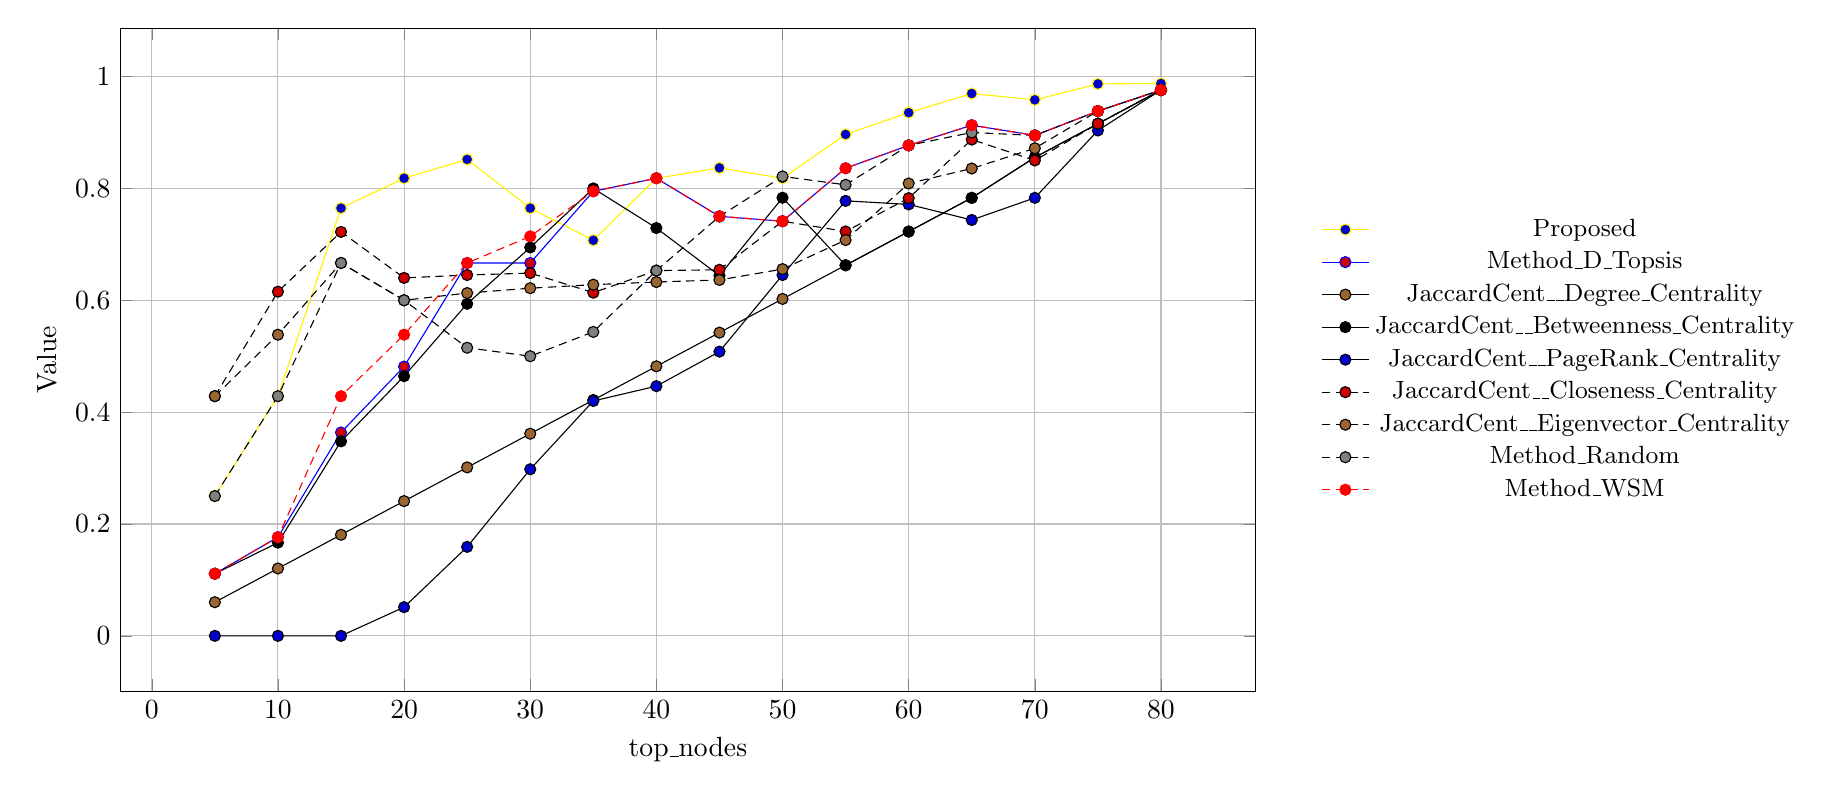
\begin{tikzpicture}
\begin{axis}[
    width=16cm,
    height=10cm,
    xlabel={top\_nodes},
    ylabel={Value},
    grid=major,
    legend style={
        at={(1.05,0.5)},
        anchor=west,
        font=\small,
        draw=none,
        cells={align=left},
    },
]
% Proposed
\addplot+[color=yellow, mark=*] coordinates {
(5.0,0.25) (10.0,0.4285714285714285) (15.0,0.7647058823529411) (20.0,0.8181818181818182) (25.0,0.8518518518518519) (30.0,0.7647058823529411) (35.0,0.7073170731707317) (40.0,0.8181818181818182) (45.0,0.8367346938775511) (50.0,0.8181818181818182) (55.0,0.896551724137931) (60.0,0.935483870967742) (65.0,0.9696969696969696) (70.0,0.9583333333333334) (75.0,0.986842105263158) (80.0,0.9876543209876544) };
\addlegendentry{Proposed}

% Method\_D\_Topsis
\addplot+[color=blue, mark=*] coordinates {
(5.0,0.1111111111111111) (10.0,0.1764705882352941) (15.0,0.3636363636363636) (20.0,0.4814814814814814) (25.0,0.6666666666666666) (30.0,0.6666666666666666) (35.0,0.7948717948717948) (40.0,0.8181818181818182) (45.0,0.75) (50.0,0.7413793103448276) (55.0,0.8360655737704918) (60.0,0.8769230769230769) (65.0,0.9130434782608696) (70.0,0.8947368421052632) (75.0,0.9382716049382716) (80.0,0.9759036144578314) };
\addlegendentry{Method\_D\_Topsis}

% JaccardCent\_\_Degree\_Centrality
\addplot+[color=black, mark=*] coordinates {
(5.0,0.0602409638554216) (10.0,0.1204819277108433) (15.0,0.180722891566265) (20.0,0.2409638554216867) (25.0,0.3012048192771084) (30.0,0.3614457831325301) (35.0,0.4216867469879518) (40.0,0.4819277108433735) (45.0,0.5421686746987951) (50.0,0.6024096385542169) (55.0,0.6626506024096386) (60.0,0.7228915662650602) (65.0,0.7831325301204819) (70.0,0.8554216867469879) (75.0,0.9156626506024096) (80.0,0.9759036144578314) };
\addlegendentry{JaccardCent\_\_Degree\_Centrality}

% JaccardCent\_\_Betweenness\_Centrality
\addplot+[color=black, mark=*] coordinates {
(5.0,0.1111111111111111) (10.0,0.1666666666666666) (15.0,0.3478260869565217) (20.0,0.4642857142857143) (25.0,0.59375) (30.0,0.6944444444444444) (35.0,0.8) (40.0,0.7291666666666666) (45.0,0.6440677966101694) (50.0,0.7833333333333333) (55.0,0.6626506024096386) (60.0,0.7228915662650602) (65.0,0.7831325301204819) (70.0,0.8554216867469879) (75.0,0.9156626506024096) (80.0,0.9759036144578314) };
\addlegendentry{JaccardCent\_\_Betweenness\_Centrality}

% JaccardCent\_\_PageRank\_Centrality
\addplot+[color=black, mark=*] coordinates {
(5.0,0.0) (10.0,0.0) (15.0,0.0) (20.0,0.0512820512820512) (25.0,0.1590909090909091) (30.0,0.2978723404255319) (35.0,0.42) (40.0,0.4464285714285714) (45.0,0.5081967213114754) (50.0,0.6451612903225806) (55.0,0.7777777777777778) (60.0,0.7714285714285715) (65.0,0.7435897435897436) (70.0,0.7831325301204819) (75.0,0.9036144578313252) (80.0,0.9759036144578314) };
\addlegendentry{JaccardCent\_\_PageRank\_Centrality}

% JaccardCent\_\_Closeness\_Centrality
\addplot+[color=black, mark=*] coordinates {
(5.0,0.4285714285714285) (10.0,0.6153846153846154) (15.0,0.7222222222222222) (20.0,0.64) (25.0,0.6451612903225806) (30.0,0.6486486486486487) (35.0,0.6136363636363636) (40.0,0.6530612244897959) (45.0,0.6545454545454545) (50.0,0.7413793103448276) (55.0,0.7230769230769231) (60.0,0.782608695652174) (65.0,0.8873239436619719) (70.0,0.85) (75.0,0.9156626506024096) (80.0,0.9759036144578314) };
\addlegendentry{JaccardCent\_\_Closeness\_Centrality}

% JaccardCent\_\_Eigenvector\_Centrality
\addplot+[color=black, mark=*] coordinates {
(5.0,0.4285714285714285) (10.0,0.5384615384615384) (15.0,0.6666666666666666) (20.0,0.6) (25.0,0.6129032258064516) (30.0,0.6216216216216216) (35.0,0.627906976744186) (40.0,0.6326530612244898) (45.0,0.6363636363636364) (50.0,0.6557377049180327) (55.0,0.7076923076923077) (60.0,0.8088235294117647) (65.0,0.8356164383561644) (70.0,0.8717948717948718) (75.0,0.9382716049382716) (80.0,0.9759036144578314) };
\addlegendentry{JaccardCent\_\_Eigenvector\_Centrality}

% Method\_Random
\addplot+[color=black, mark=*] coordinates {
(5.0,0.25) (10.0,0.4285714285714285) (15.0,0.6666666666666666) (20.0,0.6) (25.0,0.5151515151515151) (30.0,0.5) (35.0,0.5434782608695652) (40.0,0.6530612244897959) (45.0,0.75) (50.0,0.8214285714285714) (55.0,0.8064516129032258) (60.0,0.8769230769230769) (65.0,0.9) (70.0,0.8947368421052632) (75.0,0.9382716049382716) (80.0,0.9759036144578314) };
\addlegendentry{Method\_Random}

% Method\_WSM
\addplot+[color=red, mark=*] coordinates {
(5.0,0.1111111111111111) (10.0,0.1764705882352941) (15.0,0.4285714285714285) (20.0,0.5384615384615384) (25.0,0.6666666666666666) (30.0,0.7142857142857143) (35.0,0.7948717948717948) (40.0,0.8181818181818182) (45.0,0.75) (50.0,0.7413793103448276) (55.0,0.8360655737704918) (60.0,0.8769230769230769) (65.0,0.9130434782608696) (70.0,0.8947368421052632) (75.0,0.9382716049382716) (80.0,0.9759036144578314) };
\addlegendentry{Method\_WSM}


\end{axis}
\end{tikzpicture}

\end{document}
